\documentclass{beamer}
\usepackage[utf8]{inputenc}
\usepackage{tikz}
\usetikzlibrary{shapes.geometric, arrows}
\usepackage{graphicx}



\tikzstyle{city} = [circle, minimum width=0.5cm, minimum height=0.5cm, text centered, draw=black, fill=green!30]
\tikzstyle{process} = [rectangle, minimum width=1cm, minimum height=2cm, text centered, text width=3cm, draw=black, fill=orange!30]
\tikzstyle{arrow} = [thick,->,>=stealth]

\tikzstyle{line}=[draw, thick, -]

\title{Travelling Salesman Problem}
\usetheme{Madrid}
\usecolortheme{seahorse}
\setbeamertemplate{page number in head/foot}{}

\AtBeginSection[]
{
  \begin{frame}
    \frametitle{Table of Contents}
    \tableofcontents[currentsection]
  \end{frame}
}

\begin{document}


\author[1905113,1905114,1905117]
{\large{\textbf{Anamul Hoque Emtiaj(1905113)  \\  \and Sk. Saifullah Hafiz(1905114) \\ \and Nur Hossain Raton(1905117) }}} \\ 

%\author{A.~B \and X.~Y}

\institute[BUET]
{
 \large {Department of Computer Science and Engineering\\
  Bangladesh University of Engineering and Technology}
}
\frame{\titlepage}
\begin{frame}{Table of contents}
\tableofcontents
\end{frame}


\section{Problem Statement}
\begin{frame}{Problem Statement}
\begin{block}{Travelling Salesman Problem}
Given a set of cities and the distance between every pair of cities, the problem is to find the shortest possible route that visits every city exactly once and returns to the starting point
\end{block}

    
\end{frame}
\begin{frame}{Problem Statement}
 \begin{tikzpicture}[node distance=2cm]

 \node (start) [padding = 3cm,city] {A};
\node (start1) [city,left of = start,yshift= -2cm,xshift = -1cm] {B};
\node (start2) [city,right of = start,xshift =1cm,yshift= -2cm] {C};
\node (start3) [city,above of = start,yshift= 0.5cm] {D};
% \node (start4) [city,right of = start3,yshift= -1.5cm,xshift = -6cm] {E};


 \draw [line] (start) --node[anchor=west] {25}(start1);
\draw [line] (start1) --node[anchor=south] {30} (start2);
\draw [line] (start) --node[anchor=south] {35} (start2);
\draw [line] (start) --node[anchor=west] {20} (start3);
\draw [line] (start1) --node[anchor=east] {10} (start3);
 \draw [line] (start2) --node[anchor=west] {15} (start3);
 % \draw [line] (start3) --node[anchor=south] {1} (start4);
 % \draw [line] (start4) --node[anchor=south] {7} (start);

 
 \end{tikzpicture}
 \newline
 \newline
 
 
\end{frame}

\section{Application}

\begin{frame}{Application}
\textbf{Genetics and Biology}\\
\textit{- to optimize the order in which different genes are sequenced}\\
\\
\begin{center}

\includegraphics[width = 0.7\textwidth]{gene.jpg}\\
Image : \href{https://sapac.illumina.com/science/customer-stories/icommunity-customer-interviews-case-studies/retter-genedx-interview-dragen-bioinformatics.html}{https://bit.ly/3KyXsqz}
\end{center}
\end{frame}

\begin{frame}{Application}
\textbf{Logistics and Transportation}\\
\textit{-to optimize the delivery routes of goods, services, or people}\\
\\
\begin{center}
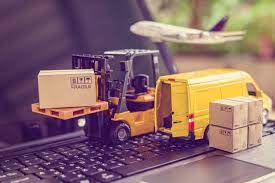
\includegraphics[width = 0.7\textwidth]{tsp1.jpg}\\
Image : \href{https://magenest.com/en/ecommerce-delivery/}{https://bit.ly/3IMfl3V}
\end{center}
\end{frame}

\begin{frame}{Application}
\textbf{Computer Wiring}\\
\textit{-connecting together computer 			         	         	              components using minimum wire length}\\


\begin{center}
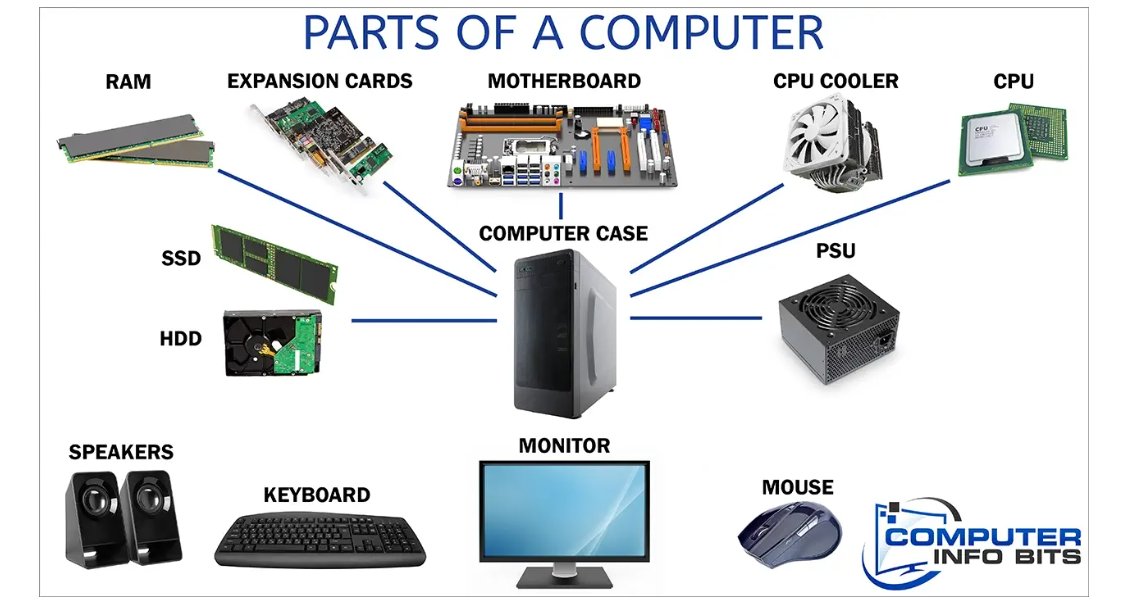
\includegraphics[width = 0.8\textwidth]{tsp.PNG}\\
Image : \href{https:https://computerinfobits.com/parts-of-computer-and-their-functions/}{https://bit.ly/3YYr44W}
\end{center}
\end{frame}

\begin{frame}{Application}

\begin{itemize}
    \item \textit{ Network Design}\\
    \item \textit{ Circuit Board Design}\\
    \item \textit{Job Sequencing}\\
    \item \textit{Airplane Scheduling}\\
  
\end{itemize}

  \item \textit{And many more ...}\\

\end{frame}


\section{Possible Implementation methods}
\begin{frame}{How to implement?}
    \begin{columns}
    \column{1\textwidth}
    \begin{figure}[h]
        \centering
        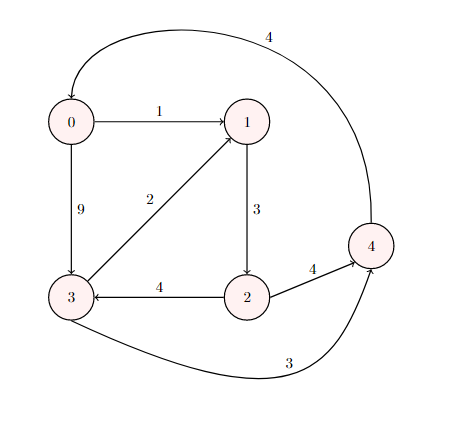
\includegraphics[scale=0.6]{g1.png}
    \end{figure}
    What will be the minimum cost?
    \end{columns}
\end{frame}

\begin{frame}{How to implement?}
    Path 1:
    \begin{columns}
    \column{0.6\textwidth}
    \begin{figure}[h]
        \centering
        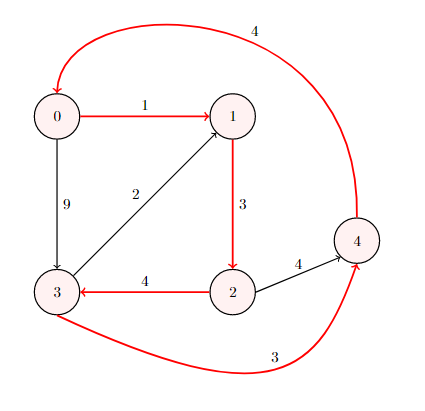
\includegraphics[scale=0.6]{g2.png}
    \end{figure}
    \column{0.4\textwidth}
    \begin{itemize}
        \item<1-> $0-1-2-3-4-0$
    \end{itemize}
    \end{columns}
    \begin{center}Cost: 1\emph{(0-1)} + 3\emph{(1-2)} + 4\emph{(2-3)} + 3\emph{(3-4)} + 4\emph{(4-0)} = 15\end{center}
\end{frame}

\begin{frame}{How to implement?}
    Path 2:
    \begin{columns}
    \column{0.6\textwidth}
    \begin{figure}[h]
        \centering
        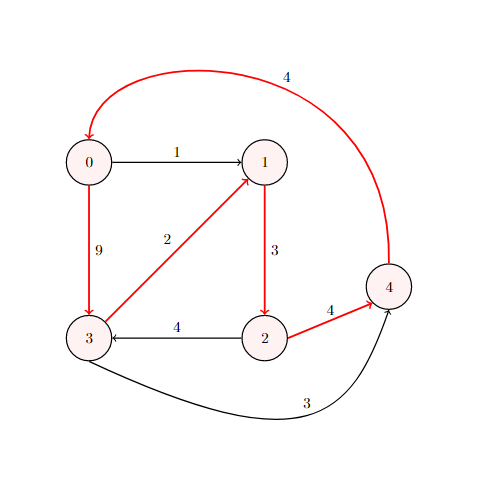
\includegraphics[scale=0.6]{g3.png}
    \end{figure}
    \column{0.4\textwidth}
    \begin{itemize}
        \item<1-> $0-3-1-2-4-0$
    \end{itemize}
    \end{columns}
    \begin{center}Cost: 9\emph{(0-3)} + 2\emph{(3-1)} + 3\emph{(1-2)} + 4\emph{(2-4)} + 4\emph{(4-0)} = 22\end{center}
\end{frame}




\begin{frame}{How to implement?}
    \begin{columns}
    \column{0.5\textwidth}
    \begin{figure}[h]
        \centering
        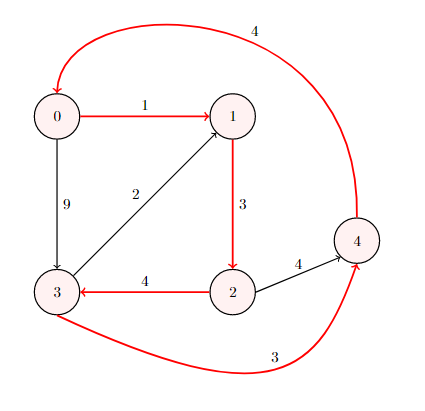
\includegraphics[scale=0.45]{g2.png}
    \end{figure}
    \column{0.5\textwidth}
    \begin{figure}[h]
        \centering
        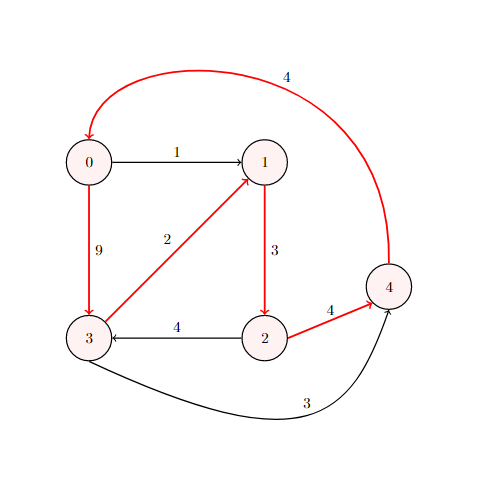
\includegraphics[scale=0.45]{g3.png}
    \end{figure}
    \end{columns}
    \begin{center}
        Here the minimal cost is 15 
    \end{center}
    \begin{itemize}
        \item A complete graph with n vertex gives n! different path combinations
        \item Which requires $O(n^2n!)$ runtime
        \item No Polynomial time solution
        \item NP-hard problem
    \end{itemize}
   
\end{frame}

\begin{frame}{How to implement?}
\begin{itemize}
    \item<1-> Others possible ways of solutions\\
        \begin{enumerate}
            \item<2-> Branch and Bound
            \item<3-> Approximation using MST
            \item<4-> Bitmask Dynamic Programming
        \end{enumerate}
    \item<5-> \alert{Here we only see Bitmask DP algorithm}
\end{itemize}
\end{frame}




\section{Implementation with Bitmask DP}
\begin{frame}{Sub Problem}
\begin{itemize}
    \item<1-> \textit{ Define a function }$f(i)$\\
    \begin{itemize}
        \item <2-> Distance for exploring the rest of the cities starting from city i.
    \end{itemize}
    \item<3-> \textit{But what is the problems? }\\
    \begin{itemize}
        \item <4-> Can't travel one city more than once.
        \item <5->Must remember which city we already visited.
    \end{itemize}
\end{itemize}
\end{frame}

\begin{frame}{Why Bit Mask?}
\begin{itemize}
    \item<1-> \textit{Use bit mask for denoting city status }\\
    \item<2-> \textit{A 32 bit integer use as mask}\\
    \begin{itemize}
        \item<3-> Bit i indicates, whether city i is already visited or not.
        \begin{enumerate}
            \item<4-> 0 for not visited.
            \item<5> 1 for visited.
        \end{enumerate}
    \end{itemize}
\end{itemize}
\end{frame}
\begin{frame}{..Cont'd Subproblem}
    \begin{itemize}
        \item<1-> \textit{ Add additional parameter mask.}\\
        \begin{itemize}
            \item<2-> Our updated function, $f(i,mask)$.
            \item<3-> i indicates present city.
            \item<4-> mask contains information about the tour.
        \end{itemize}
        \item<4-> \textit{How do we implement bit masking?}\\
    \end{itemize}
\end{frame}
\begin{frame}{Bit Masking}
    \begin{columns}
        \column{0.48\textwidth}
            If started from city 0. 
             \pause
            \begin{figure}[h]
        	\centering
        	%\caption{This caption is at the top}
        	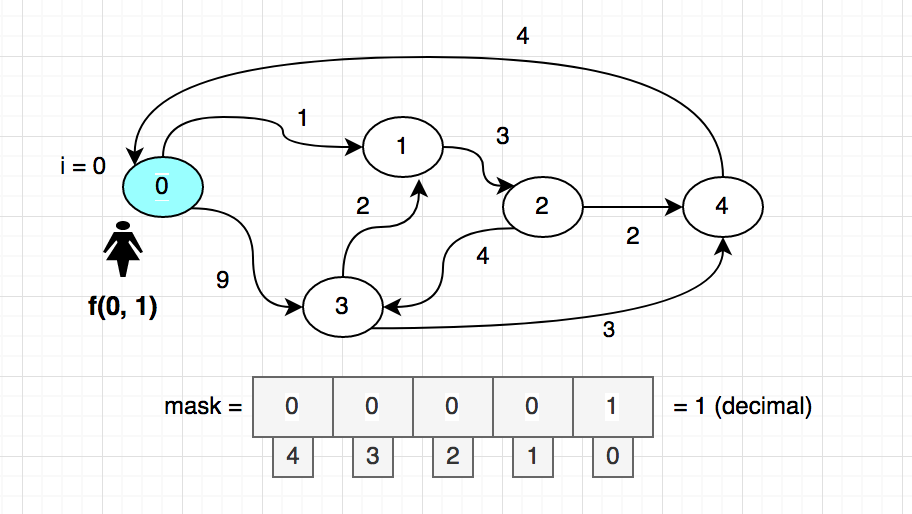
\includegraphics[scale=0.4]{s1.png}
        	\label{fig:1}
            \end{figure}
        \pause
        \column{0.48\textwidth}
            Then he goes to city 3.
             \pause
            \begin{figure}[h]
        	\centering
        	%\caption{This caption is at the top}
        	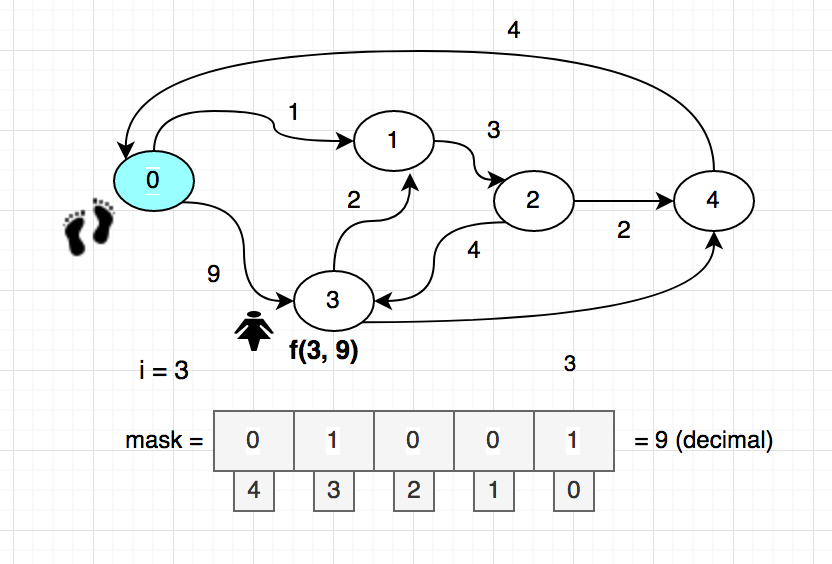
\includegraphics[scale=0.4]{s2.png}
        	\label{fig:2}
            \end{figure}
    \end{columns}
\end{frame}

\begin{frame}{Bit Masking}
    \begin{columns}
        \column{0.50\textwidth}
        \begin{figure}[h]
            \centering
            %\caption{This caption is at the top}
            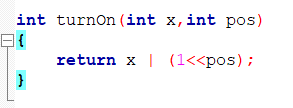
\includegraphics[scale=1]{ton.png}
            \label{fig:3}
        \end{figure}
        \column{0.20\textwidth}
        \begin{tikzpicture}
            \draw[arrow] (-6,7) -- (-4,7)
        \end{tikzpicture}
        \column{0.30\textwidth}
        Code snippet for turning on a bit
    \end{columns}
    \pause
    \begin{columns}
        \column{0.50\textwidth}
        \begin{figure}[h]
            \centering
            %\caption{This caption is at the top}
            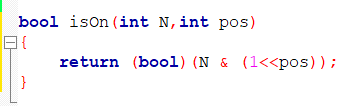
\includegraphics[scale=1]{ion.png}
            \label{fig:3}
        \end{figure}
        \column{0.20\textwidth}
        \begin{tikzpicture}
            \draw[arrow] (-6,7) -- (-4,7)
        \end{tikzpicture}
        \column{0.30\textwidth}
        Code snippet for checking a bit
    \end{columns}
\end{frame}
\begin{frame}{Recursive Formula}
    \begin{itemize}
        \item<1-> We have to solve $f(0,1)$
        \item<2-> Base case $f(i,2^{n-1})$
    \end{itemize}
    \pause
    \begin{block}{Recursive Formula}
            $f(i,2^{n-1}) = dis[i][0]$
            $f(i, mask) = min(f(j, turnOn(mask,j)) + w[i][j]) where i,j \in E$
    \end{block}
\end{frame}
\begin{frame}{Algorithm}
    \begin{figure}[h]
        \centering
        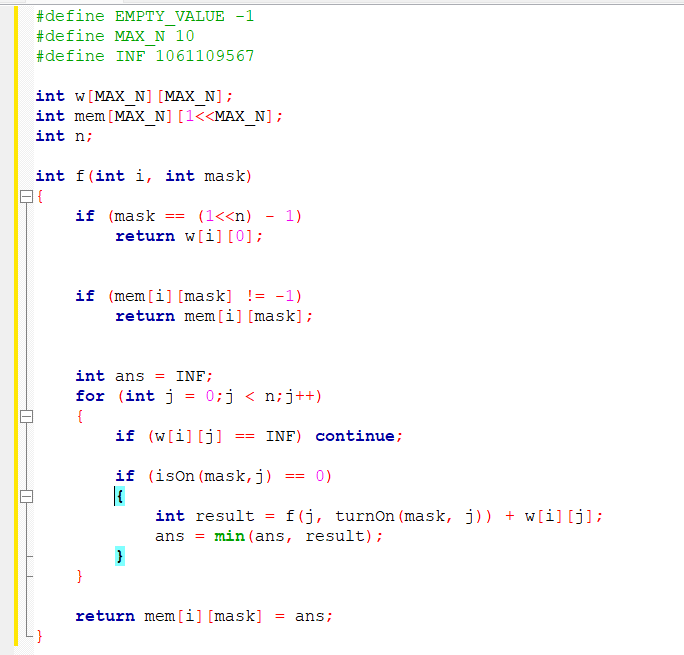
\includegraphics[scale=0.5]{algo.png}
    \end{figure}
    
\end{frame}

\begin{frame}{Time Complexity}
    \begin{itemize}
        \item<1-> For n city mask value can be 0 to $2^n$.
        \item<2-> So total $n*2^n$ states possible.
        \item<3-> Total Run time: $O(n^2*2^n)$ 
    \end{itemize}
\end{frame}

\begin{frame}
    \begin{center}
        {\Huge Thank you}
    \end{center}
\end{frame}
\begin{frame}
    \begin{center}
        {\Huge Any Question?}
    \end{center}
\end{frame}
\end{document}

